%\selectlanguage{czech}
\chapter{Možné způsoby záchrany}
\label{Mozne_zpusoby_zachrany}
%% -------------------------------------------------- %%
\def\figurename{Obr.} % Figure name
\def\tablename{Tab.} % Table name
\def\figureautorefname{obr.} % Autoreference 
\def\tableautorefname{tab.} % Autoreference
\def\chapterautorefname{kapitola} % Autoreference
%% -------------------------------------------------- %%

V následující kapitole si ukážeme možné způsoby záchrany. Záchranu budeme provádět pomocí kladkostroje. Kladkostroje se dělí podle účinnosti. 

\subsection*{Stanovení účinnosti kladkostroje}

Kladkostroj snižuje úsilí potřebné k vytažení záchraňovaného. 

\section{Kladkový efekt}

Budeme-li uvažovat břemeno zavěšené na laně procházející kladkou zavěšenou nad tímto břemenem, bude platit 2. Newtonův zákon "Síla působící na těleso o hmotnosti \textit{m} uvádí těleso do rovnoměrně zrychleného pohybu se zrychlením \textit{a}.", tedy jakákoliv síla působící na jeden konec lana se přenese na druhý konec lana.

Pokud břemeno zavěšené na laně váží 100\,kg, musí na druhé straně lana udržet, taktéž 100\,kg (viz~\autoref{Obr:pulley_system}). Každý pramen lana vyvine tah 100\,kg, takže kladka nese 200\,kg.

%% -------------------------------------------------- %%
%% -------------------- Picture --------------------- %%
%% -------------------------------------------------- %%
\begin{figure}[!hbt]
    \centering
    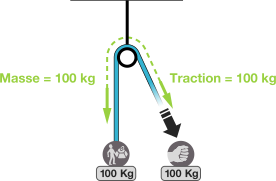
\includegraphics[width=10.0cm]{Figures/PulleySystem/pulley_system.pdf}
    \caption[Kladkový efekt]{Kladkový efekt (schéma převzato ze zdroje \cite{Petzl_2022})}
    \label{Obr:pulley_system}
\end{figure} 
%% -------------------------------------------------- %%

Tato teorie platí pouze pro ideální kladkostroj s účinností 100\%, která reálně neexistuje. Ve skutečnosti se dokážeme pohybovat v rozmezí od 50\% do 98\%. Pro zjednodušenní výpočtů budu pracovat s účinností 100\%.

Účinnost tj. síla značená (E) taženého systému udává multiplikační faktor síly, který můžeme na lano vyvinout. Pokud jsme na laně schopni utáhnout 20\,kg systém 3:1 umožní zvednou 60\,kg. Tohoto snížení se dosáhne zvýšením množství taženého lana. Uvažujeme-li ideální stav, tedy 100\% účinnost systému, potřebujeme k vytažení zátěže o 1\,m se systémem 3:1 vytáhnout 3\,m lana.

Účinnost (E) taženého systému lze vypočítat sečtením účinků každé kladky. Pokud máme kladkostroje se sudým číslem, jedná se o formu kladkostroje se zatížením ukotveným nahoře. V našem případě budeme využívat kladkostroje s lichým číslem, tedy se zatížením dole. Zaměřím se na kladkostroj 3:1, 5:1 a 7:1 \cite{Petzl_2022}.

\section{Kladkostroje}

Pro určení mechanické účinnosti systému slouží T-metoda, neboli metoda sčítání napětí. Jedná se o výpočet mechanické účinnosti lana a kladky. K určení T-metody stačí pouze následovat 4. kroky:

1. Vedle taženého lana zapíšeme T1.

2. Vedle každé kladky si zakreslíme tři čáry, tyto čáry budou značit vstup do kladky, kladku a výstup z kladky. Vždy platí rovnováha sil, tedy síly co vstoupí do kladky musí i vystoupit.

3. Doplníme prázdné řádky.

4. Po doplnění všech řádek zjistíme mechanickou účinnost systému \cite{rope_rescue_web_calculating_MA_T_system} (viz Obr. Rozložení sil).
\newpage
\subsection{Systém 1:1}
%% -------------------------------------------------- %%
%% -------------------- Pictures --------------------- %%
%% -------------------------------------------------- %%
\begin{figure}[h]
    \centering
    \subcaptionbox{Sestrojení kladkostroje\label{Obr:1:1_Pulley_system}}{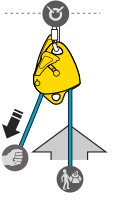
\includegraphics[width=5.0cm]{Figures/1_1/1_haul_system_1_1.pdf}}%
    \hfill % Seperation
    \subcaptionbox{Schéma kladkostroje\label{Obr:1:1_diagram}}{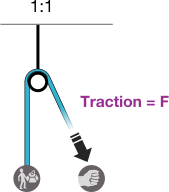
\includegraphics[width=5.0cm]{Figures/1_1/2_haul_system_1_1.pdf}}%
    \\ % Line break
    \subcaptionbox{Rozložení sil\label{Obr:1:1_forces_distribution}}{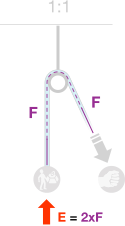
\includegraphics[width=5.0cm]{Figures/1_1/3_haul_system_1_1.pdf}}%
    \caption[Kladkostroj 1:1]{Kladkostroj 1:1 (schéma převzato ze zdroje \cite{Petzl_2022})}
    \label{Obr:1:1}
\end{figure}
%% -------------------------------------------------- %%

\newpage
\subsection{Systém 2:1}
%% -------------------------------------------------- %%
%% -------------------- Pictures --------------------- %%
%% -------------------------------------------------- %%
\begin{figure}[h]
    \centering
    \subcaptionbox{Sestrojení kladkostroje\label{Obr:2:1_Pulley_system}}{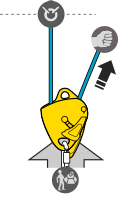
\includegraphics[width=5.0cm]{Figures/2_1/1_haul_system_2_1.pdf}}%
    \hfill % Seperation
    \subcaptionbox{Schéma kladkostroje\label{Obr:2:1_diagram}}{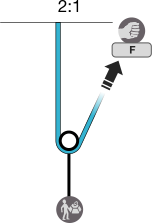
\includegraphics[width=5.0cm]{Figures/2_1/2_haul_system_2_1.pdf}}%
    \\ % Line break
    \subcaptionbox{Rozložení sil\label{Obr:2:1_forces_distribution}}{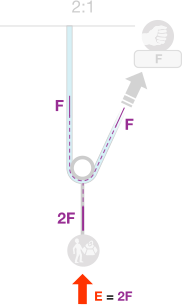
\includegraphics[width=5.0cm]{Figures/2_1/3_haul_system_2_1.pdf}}%
    \caption[Kladkostroj 2:1]{Kladkostroj 2:1 (schéma převzato ze zdroje \cite{Petzl_2022})}
    \label{Obr:2:1}
\end{figure}
%% -------------------------------------------------- %%

\newpage
\subsection{Systém 3:1}
%% -------------------------------------------------- %%
%% -------------------- Pictures --------------------- %%
%% -------------------------------------------------- %%
\begin{figure}[h]
    \centering
    \subcaptionbox{Sestrojení kladkostroje\label{Obr:3:1_Pulley_system}}{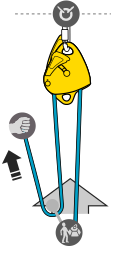
\includegraphics[width=4.0cm]{Figures/3_1/1_haul_system_3_1.pdf}}%
    \hfill % Seperation
    \subcaptionbox{Zobrazení sestrojeného kladkostroje\label{Obr:3:1_Figure_pulley_system}}{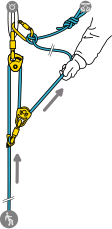
\includegraphics[width=5.0cm]{Figures/3_1/2_haul_system_3_1.pdf}}%
    \\ % Line break
    \subcaptionbox{Schéma kladkostroje\label{Obr:3:1_diagram}}{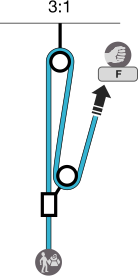
\includegraphics[width=4.0cm]{Figures/3_1/3_haul_system_3_1.pdf}}%
    \hfill % Seperation
    \subcaptionbox{Rozložení sil\label{Obr:3:1_forces_distribution}}{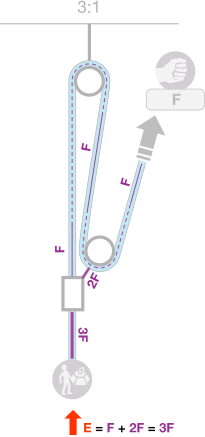
\includegraphics[width=4.0cm]{Figures/3_1/4_haul_system_3_1.pdf}}%
    \caption[Kladkostroj 3:1]{Kladkostroj 3:1 (schéma převzato ze zdroje \cite{Petzl_2022})}
    \label{Obr:3:1}
\end{figure}
%% -------------------------------------------------- %%

\newpage
\subsection{Systém 4:1}
%% -------------------------------------------------- %%
%% -------------------- Pictures --------------------- %%
%% -------------------------------------------------- %%
\begin{figure}[h]
    \centering
    \subcaptionbox{Sestrojení kladkostroje\label{Obr:4:1_Pulley_system}}{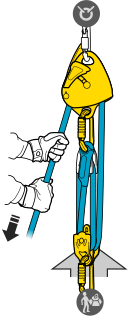
\includegraphics[width=4.0cm]{Figures/4_1/1_haul_system_4_1.pdf}}%
    \hfill % Seperation
    \subcaptionbox{Zobrazení sestrojeného kladkostroje\label{Obr:4:1_Figure_pulley_system}}{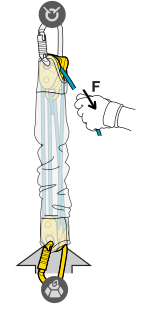
\includegraphics[width=4.0cm]{Figures/4_1/2_haul_system_4_1.pdf}}%
    \\ % Line break
    \subcaptionbox{Schéma kladkostroje\label{Obr:4:1_diagram}}{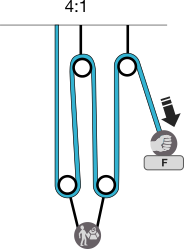
\includegraphics[width=4.0cm]{Figures/4_1/3_haul_system_4_1.pdf}}%
    \hfill % Seperation
    \subcaptionbox{Rozložení sil\label{Obr:4:1_forces_distribution}}{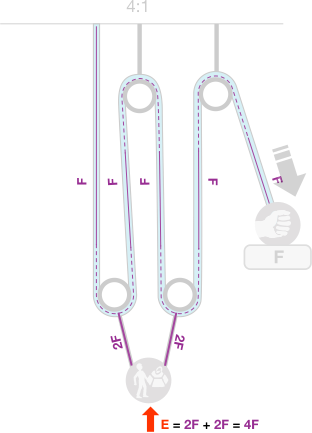
\includegraphics[width=4.0cm]{Figures/4_1/4_haul_system_4_1.pdf}}%
    \caption[Kladkostroj 4:1]{Kladkostroj 4:1 (schéma převzato ze zdroje \cite{Petzl_2022})}
    \label{Obr:4:1}
\end{figure}
%% -------------------------------------------------- %%

\newpage
\subsection{Systém 5:1}
%% -------------------------------------------------- %%
%% -------------------- Pictures --------------------- %%
%% -------------------------------------------------- %%
\begin{figure}[h]
    \centering
    \subcaptionbox{Sestrojení kladkostroje\label{Obr:5:1_Pulley_system}}{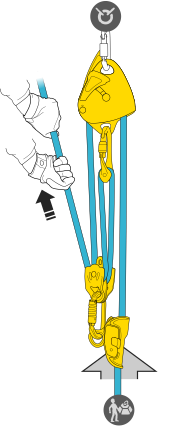
\includegraphics[width=4.0cm]{Figures/5_1/1_haul_system_5_1.pdf}}%
    \hfill % Seperation
    \subcaptionbox{Zobrazení sestrojeného kladkostroje\label{Obr:5:1_Figure_pulley_system}}{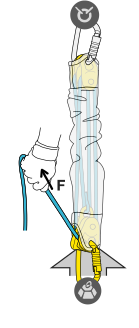
\includegraphics[width=4.0cm]{Figures/5_1/2_haul_system_5_1.pdf}}%
    \\ % Line break
    \subcaptionbox{Schéma kladkostroje\label{Obr:5:1_diagram}}{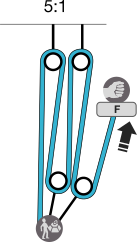
\includegraphics[width=4.0cm]{Figures/5_1/3_haul_system_5_1.pdf}}%
    \hfill % Seperation
    \subcaptionbox{Rozložení sil\label{Obr:5:1_forces_distribution}}{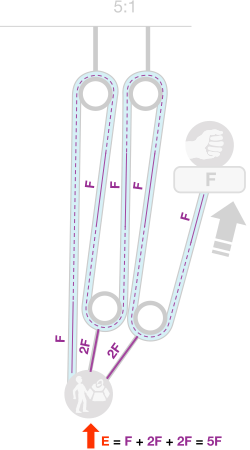
\includegraphics[width=4.0cm]{Figures/5_1/4_haul_system_5_1.pdf}}%
    \caption[Kladkostroj 5:1]{Kladkostroj 5:1 (schéma převzato ze zdroje \cite{Petzl_2022})}
    \label{Obr:5:1}
\end{figure}
%% -------------------------------------------------- %%

\newpage
\subsection{Systém 7:1}
%% -------------------------------------------------- %%
%% -------------------- Pictures --------------------- %%
%% -------------------------------------------------- %%
\begin{figure}[h]
    \centering
    \subcaptionbox{Sestrojení kladkostroje\label{Obr:7:1_Pulley_system}}{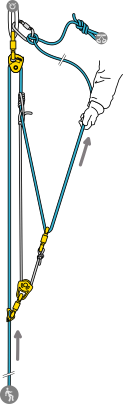
\includegraphics[width=4.0cm]{Figures/7_1/1_haul_system_7_1.pdf}}%
    \hfill % Seperation
    \subcaptionbox{Schéma kladkostroje\label{Obr:7:1_diagram}}{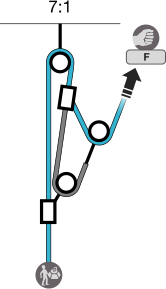
\includegraphics[width=4.0cm]{Figures/7_1/2_haul_system_7_1.pdf}}%
    \\ % Line break
    \subcaptionbox{Rozložení sil\label{Obr:7:1_forces_distribution}}{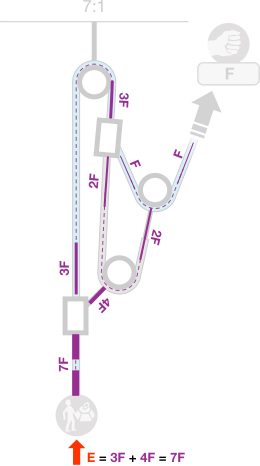
\includegraphics[width=4.0cm]{Figures/7_1/3_haul_system_7_1.pdf}}%
    \caption[Kladkostroj 7:1]{Kladkostroj 7:1 (schéma převzato ze zdroje \cite{Petzl_2022})}
    \label{Obr:7:1}
\end{figure}
%% -------------------------------------------------- %%
\section{Popis kladkostrojů}
\subsection{Systém volné kladky "Loserolle"}

Tato technika je využívána zejména při záchraně na ledovci. Nejjednoduší použití této metody je pokud je lezec při vědomí. Pokud je lezec zraněný nebo není při vědomí musíme se nejdříve k lezci slanit a až poté jej vytahovat za pomocí kladky nahoru. 
\\
\\
Postup:

1. Zřídíme stanoviště - vykopeme díru například pro vložení cepínu. Na topůrko cepínu uvážeme liščí smyčkou sešitou smyčku (viz~\autoref{Obr:Snow_anchor}). Následně cepín zakopeme a pomocí prusíku, který máme navázaný na laně uvolníme ze sebe zátěž a přeneseme ji na nově vybudované stanoviště.

2. Na volném prameni lana umístíme 3\,m prusík pro sebezajištění.

3. Na volném prameni dojdeme na kraj trhliny, celou dobu jsme jištěni prusíkem. Na volném prameni lana spustíme karabinu (kladku) k zachraňovanému lezci, který si karabinu cvakne do sedáku.

4. Prusík, který posloužil pro odtížení váhy lezce bude sloužit jako zajištění vytahovaného lana, takový to jednoduchý kladkostroj by fungoval s účinností systému 2:1 (viz~\autoref{Obr:Crevasse_2:1}). 

5. Pokud bychom volné lano ve zřízeném stanovišti zajistili prusíkem, tiblocem nebo microtraxtionem a dále použili prusík s karabinou popřípadě tibloc s karabinou a kladkou vytvořili bychom systém 6:1 (viz~\autoref{Obr:Crevasse_6:1}). Další možností je vytvořit systém 3:1 (viz~\autoref{Obr:Crevasse_3:1}) nebo 7:1 (viz~\autoref{Obr:Crevasse_7:1}) \cite{climbing_school_2022}.
\\
\\
Nejčastější chyby:

1. Celý systém je zajištěn pouze přes jeden prusík.

2. Chybné nastavení délek prusíků.

3. Překřížení pramenů lana v systému.
%% -------------------------------------------------- %%
%% -------------------- Pictures --------------------- %%
%% -------------------------------------------------- %%
\begin{figure}[h]
    \centering
    {\includegraphics[width=8.0cm]{Figures/Crevasse/Snow_anchor.png}}%
    \caption[Snehova_kotva]{Sněhová kotva (schéma převzato ze zdroje \cite{Petzl_2022})}
    \label{Obr:Snow_anchor}
\end{figure}
%% -------------------------------------------------- %%
%% -------------------- Pictures --------------------- %%
%% -------------------------------------------------- %%
\begin{figure}[h]
    \centering
    {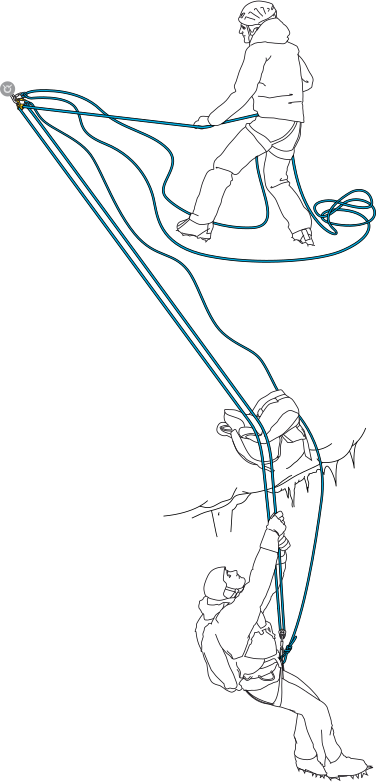
\includegraphics[width=8.0cm]{Figures/Crevasse/1_Petzl_Crevasse_haul_system_2_1.pdf}}%
    \caption[Crevasse 2:1]{Záchrana z ledovcové trhliny 2:1 (schéma převzato ze zdroje \cite{Petzl_2022})}
    \label{Obr:Crevasse_2:1}
\end{figure}
%% -------------------------------------------------- %%
%% -------------------- Pictures --------------------- %%
%% -------------------------------------------------- %%
\begin{figure}[h]
    \centering
    {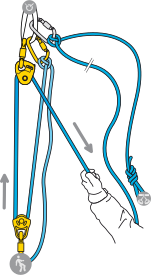
\includegraphics[width=4.0cm]{Figures/Crevasse/1_Petzl_Crevasse_haul_system_2_1_detail.pdf}}%
    \caption[Crevasse 2:1 detail]{Detail kladkostroje pro záchranu z ledovcové trhliny 2:1 (schéma převzato ze zdroje \cite{Petzl_2022})}
    \label{Obr:Crevasse_2:1_detail}
\end{figure}
%% -------------------------------------------------- %%
%% -------------------- Pictures --------------------- %%
%% -------------------------------------------------- %%
\begin{figure}[h]
    \centering
    {\includegraphics[width=8.0cm]{Figures/Crevasse/2_Petzl_Crevasse_haul_system_3_1.pdf}}%
    \caption[Crevasse 3:1]{Záchrana z ledovcové trhliny 3:1 (schéma převzato ze zdroje \cite{Petzl_2022})}
    \label{Obr:Crevasse_3:1}
\end{figure}
%% -------------------------------------------------- %%
%% -------------------- Pictures --------------------- %%
%% -------------------------------------------------- %%
\begin{figure}[h]
    \centering
    {\includegraphics[width=4.0cm]{Figures/Crevasse/2_Petzl_Crevasse_haul_system_3_1_detail.pdf}}%
    \caption[Crevasse 3:1 detail]{Detail kladkostroje pro záchranu z ledovcové trhliny 3:1 (schéma převzato ze zdroje \cite{Petzl_2022})}
    \label{Obr:Crevasse_3:1_detail}
\end{figure}
%% -------------------------------------------------- %%
%% -------------------- Pictures --------------------- %%
%% -------------------------------------------------- %%
\begin{figure}[h]
    \centering
    {\includegraphics[width=10.0cm]{Figures/Crevasse/3_Crevasse_haul_system_6_1.jpg}}%
    \caption[Crevasse 6:1]{Záchrana z ledovcové trhliny 6:1 (schéma převzato ze zdroje \cite{stock_alpine_2022})}
    \label{Obr:Crevasse_6:1}
\end{figure}
%% -------------------------------------------------- %%
%% -------------------- Pictures --------------------- %%
%% -------------------------------------------------- %%
\begin{figure}[h]
    \centering
    {\includegraphics[width=8.0cm]{Figures/Crevasse/4_Petzl_Crevasse_haul_system_7_1.pdf}}%
    \caption[Crevasse 7:1]{Záchrana z ledovcové trhliny 7:1 (schéma převzato ze zdroje \cite{Petzl_2022})}
    \label{Obr:Crevasse_7:1}
\end{figure}
%% -------------------------------------------------- %%
%% -------------------- Pictures --------------------- %%
%% -------------------------------------------------- %%
\begin{figure}[h]
    \centering
    {\includegraphics[width=4.0cm]{Figures/Crevasse/4_Petzl_Crevasse_haul_system_7_1_detail.pdf}}%
    \caption[Crevasse 7:1 detail]{Detail kladkostroje pro záchranu z ledovcové trhliny 7:1 (schéma převzato ze zdroje \cite{Petzl_2022})}
    \label{Obr:Crevasse_7:1_detail}
\end{figure}
%% -------------------------------------------------- %%